繪製直方圖:(i)將橫座標改機率值,(ii)縱座標標籤設計為”probability”,(iii)標題為”Histogram of Poi(10.2)”

\begin{lstlisting}[language=R]
> hist(x, ylab='probability', main='Histogram of Poi(10.2)'
    , pro=T)
\end{lstlisting}

\begin{figure}[h]
    \centering
    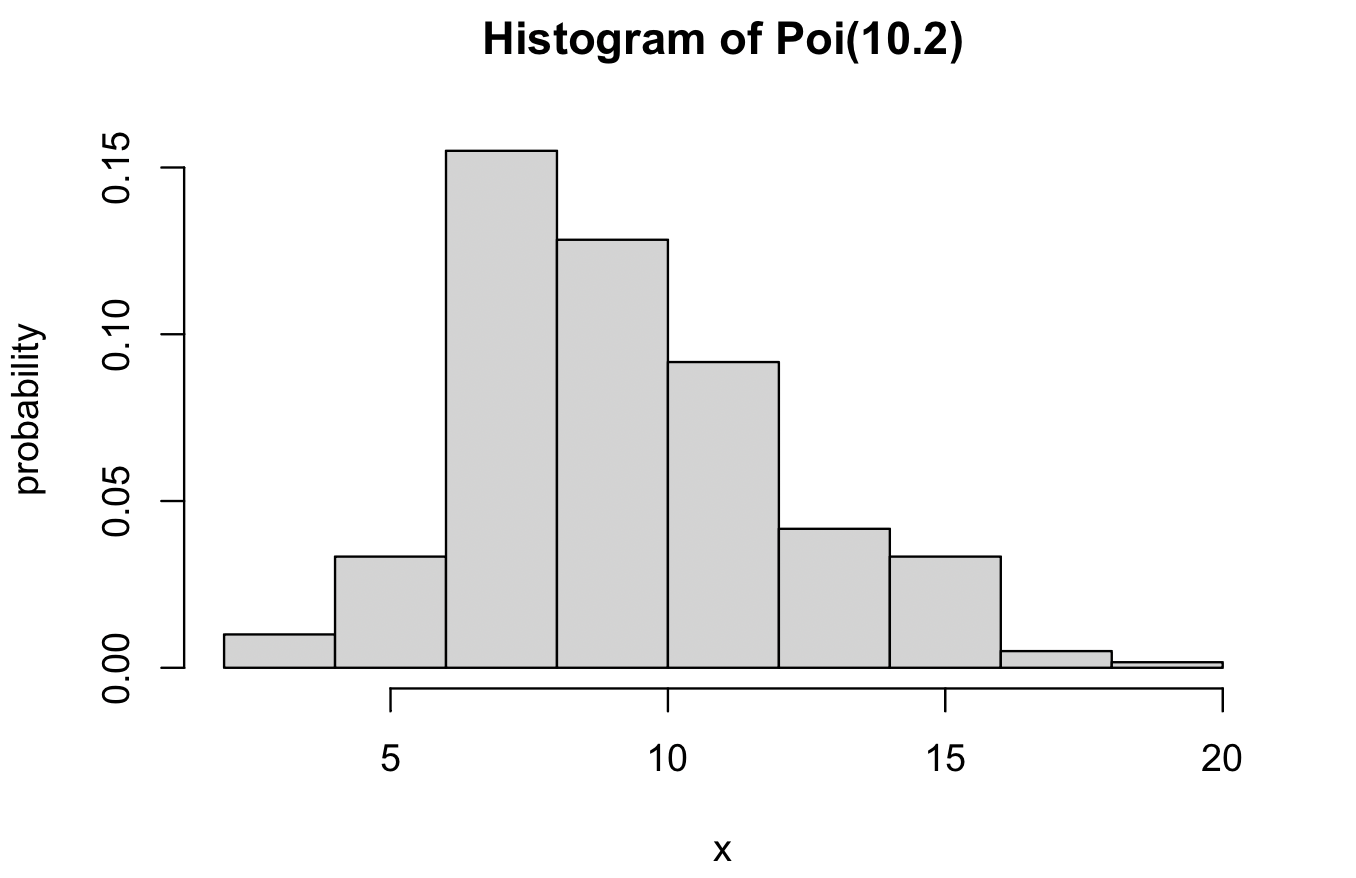
\includegraphics[width=10cm, height=7cm]{figures/Histogram.png}
    \caption{Histogram of Poi(10.2)}
    \label{fig:1}
\end{figure}